\chapter{KNN}

En este capítulo vamos a presentar el primero de los muchos algoritmos de clasificación que vamos a estudiar a lo largo del curso, elegimos este algoritmo por ser muy simple de entender y porque suele dar muy buenos resultados aun en problemas complejos, es un algoritmo que permite realizar tareas tanto de clasificación como de regresión y que también es usado luego en otros algoritmos como parte del proceso. Mencionamos todo esto para destacar la importancia que tiene y la necesidad de conocerlo en detalle. 

El algoritmo se denomina KNN (K-Nearest-Neighbors) ya que se basa en encontrar para un determinado punto sus K-vecinos mas cercanos. Asumimos que nuestro set de datos está formado por un conjunto de $m$ puntos en $n$ dimensiones siendo todos los valores numéricos. 

Para poder usar KNN hay que definir dos cosas: la métrica a usar para calcular las distancias y el valor de $k$ es decir cuantos vecinos vamos a considerar. A modo de ejemplo veamos un caso en el cual usamos KNN para clasificación usando la distancia euclidiana.

\begin{figure}[!htb]
\centering
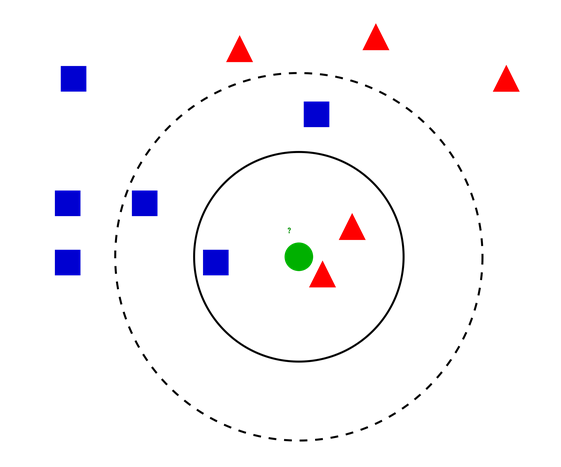
\includegraphics[width=2in]{figures/knn-fig-1.png}
\caption{KNN.}
\label{fig10}
\end{figure}

\begin{table}[!hbt]
\center{
\begin{tabular}{|c|c|c|}\hline
K & P(Blue) & P(Red)\\ \hline\hline
1 & 0 & 1 \\
3  & 1/3 & 2/3  \\
5 & 3/5 & 2/5 \\ \hline
\end{tabular}
}
\vskip 0.25cm
\caption{Ejemplo KNN.}
\end{table}

La tabla nos muestra para diferentes valores de $k$ cual es la probabilidad de cada una de las clases, en nuestro caso rojo o azul. Como podemos ver para el punto verde si $k=1$ tomamos únicamente el punto mas cercano y determinamos que la clase es la de dicho punto, en nuestro caso rojo con probabilidad 1 y por lo tanto la probabilidad de azul es cero. Si tomamos $k=3$ entonces tomamos los tres vecinos mas cercanos, dos son rojos y uno es azul por lo tanto la probabilidad de rojo es 2/3 y la probabilidad de azul es 1/3. Finalmente con $k=5$ tenemos tres puntos azules y dos rojos por lo que ahora la clase mas probable es azul con probabilidad 3/5 y rojo tiene probabilidad 2/5.

Cuando queremos simplemente clasificar un punto cuya clase no conocemos no hacen falta las probabilidades podemos simplemente asignarlo a la clase con mayoría entre los k-vecinos del punto. 

Si nuestro problema es de regresión entonces podemos predecir para nuestro punto el promedio de los valores de los k-vecinos mas cercanos.

Con este sencillo esquema tenemos un algoritmo muy útil tanto para problemas de clasificación como de regresión, pero KNN no solo se usa como algoritmo de clasificación y regresión sino que es también parte fundamental de otros algoritmos. Por ejemplo podemos usar KNN en el marco de un sistema de recomendaciones, tomando las $k$ películas mas similares a las que le gustan al usuario para recomendarlas o tomando los $k$ usuarios mas parecidos al usuario para recomendarle películas que  estos hayan visto. Es por este motivo que KNN es un algoritmo sumamente importante y que estudiaremos en detalle.

\section{La Métrica a emplear}

La métrica a emplear para las distancias en KNN es sumamente importante, puede usarse cualquier métrica que cumpla las siguientes propiedades:
\begin{enumerate}
\item $d(x,y)\geq0$
\item $d(x,y) = d(y,x)$
\item $d(x,y)\leq d(x,z)+d(z,y)$
\end{enumerate}

Las tres propiedades son conocidas, una distancia debe ser positiva, simétrica y debe cumplir la desigualdad triangular.
Dado que vamos a usar distancias no solo en KNN sino en muchos algoritmos a lo largo del curso es conveniente hacer un listado de las distancias mas populares y sus definiciones para poder mencionar en que casos es posible usarlas.

\subsection{Distancia Minkowsky} La distancia mas general es la llamada distancia de Minkowsky cuya definición es la siguiente:

$$(\sum_{i}^{n}\lvert x_i-y_i  \rvert^p)^{\frac{1}{p}}$$

Cuando $p=2$ la distancia Minkowsky es la conocida distancia euclideana que es sin dudas la mas utilizada. Hay otros tres casos interesantes de esta distancia:

\subsection{Distancia Manhattan} En esta distancia $p=1$, la distancia Manhattan se llama así porque es la forma de calcular distancias en una ciudad con forma de grilla en la cual solo nos podemos mover por las calles en forma horizontal y vertical, la distancia entre dos puntos es entonces la sumatoria de la diferencia entre todas sus coordenadas.

\begin{figure}[!htb]
\centering
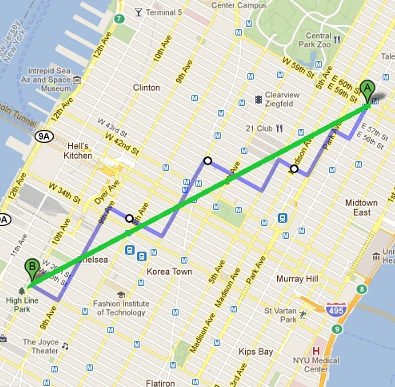
\includegraphics[width=2in]{figures/manhattan-fig.png}
\caption{Distancia Manhattan vs Distancia Euclideana.}
\label{fig11}

\end{figure}

\subsection{Distancia de Hamming o Norma $l_0$} Esta es la distancia de Minkowsky cuando $p=0$, en este caso la distancia entre dos puntos es igual a la cantidad de elementos en las cuales difieren los vectores. La distancia de Hamming en general se define y usa para vectores binarios, formados por ceros y unos pero la definición puede extenderse a vectores con valores arbitrarios contando simplemente en cuantas dimensiones los valores de los vectores son diferentes.

\begin{figure}[!htb]
\centering
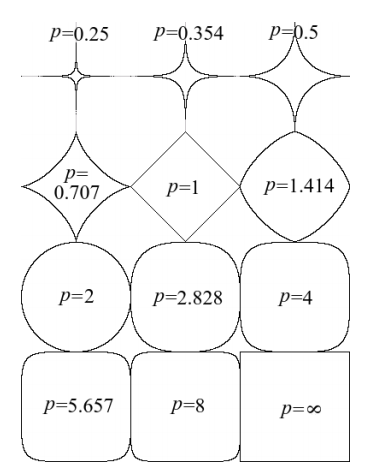
\includegraphics[width=3in]{figures/balls-fig-1}

\caption{Puntos a distancia=1 del origen para diferentes valores de $p$ en la distancia Minkowsky, observar que la distancia euclideana ($p=2$) es invariante a la rotación lo cual la hace tan popular}
\label{fig:minkowsky}
\end{figure}


\subsection{Norma $l_{\infty}$} En este caso $p=\infty$ y la distancia equivale a la diferencia mas grande entre dos elementos cualesquiera entre los vectores. Esto es fácil de ver ya que a medida que aumentamos $p$ en la distancia Minkowsky solo las coordenadas con mayor diferencia tienen peso en la distancia final, en el límite la única coordenada que realmente cuenta es la de mayor distancia.

Sean por ejemplo los siguientes vectores:

\begin{verbatim}
X = (1, 0, 2, 4)
Y = (1, 2, 1, 1)
\end{verbatim}

La distancia de Hamming entre los vectores es 3 porque difieren en tres de las 4 dimensiones. La distancia Manhattan es 6 que es la sumatoria de las distancias entre cada dimensión, la distancia euclideana es $\sqrt{14}$ y finalmente la norma $l_{\infty}$ es 3 que es la mayor diferencia entre las coordenadas de los vectores.


\subsection{Distancia de Mahalanobis}

La distancia de Mahalanobis es útil cuando tenemos atributos (features) que están correlacionados. Consideremos por ejemplo el gráfico de la figura ~\ref{fig:malahanobis}. Como podemos ver hay una correlación entre los ejes X e Y, los dos puntos marcados con las X rojas están dentro del mismo percentil de variabilidad de cada uno de sus ejes. En otras palabras en una escala relativa a la variabilidad de cada eje los dos puntos deberían estar a igual distancia del origen.

\begin{figure}[!htb]
\centering
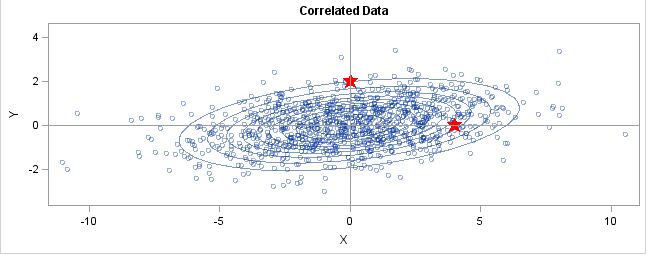
\includegraphics[width=5in]{figures/mahalanobis-fig.png}
\caption{Distancia de Mahalanobis.}
\label{fig:malahanobis}

\end{figure}

La distancia de Mahalanobis es aquella que teniendo en cuenta la variabilidad de cada uno de los atributos logra que puntos que están dentro del mismo percentil de variación para su atributo queden a la misma distancia. La fórmula para la distancia de Mahalanobis es:

$$D(x,y) = \sqrt{(x-y)S^{-1}(x-y)}$$

Donde "S" es la matriz de covarianza. La matriz de covarianza se define como aquella matriz que tiene en la diagonal la varianza de cada uno de los atributos y en los elementos $A_{ij}$ la covarianza entre los atributos "i" y "j". La matriz de covarianza se define de la siguiente forma:

$$ cov(x,y) = \frac{1}{n} \sum_{i=1}^{n} (x_i-\overline{x})(y_i-\overline{y})$$

Hay que destacar que cuando la matriz de covarianza es la identidad la distancia de Mahalanobis es igual a la distancia euclideana.

\subsection{Distancia Coseno} La distancia coseno mide la distancia entre dos vectores como el ángulo entre los mismos. Recordemos que el coseno entre dos vectores puede calcularse de la siguiente forma:

$$\cos \theta = \frac{<X,Y>}{||X|| ||Y||}$$

Es decir el producto interno entre los vectores dividido el producto de sus normas. La distancia coseno es entonces:

$$\theta = \arccos \frac{<X,Y>}{||X|| ||Y||}$$

Notemos que el coseno es una medida de semejanza (a mayor coseno mas chico el ángulo entre los vectores) mientras que el ángulo es una medida de distancia. En muchos algoritmos vamos a usar esta dualidad entre semejanzas y distancias calculando unas u otras según sea necesario.

Observemos también que si los vectores están normalizados el coseno entre los mismos puede calcularse simplemente como el producto interno entre los vectores, esta propiedad también será muy usada a lo largo del curso.

La distancia coseno se usa cuando lo que importa es la dirección en la que apuntan los vectores y no la magnitud de los mismos. Es una distancia muy usada en textos, por ejemplo en el modelo Bag of Words ya que lo que nos importa es la diferencia semántica entre los textos y no si un texto es mas largo que el otro. Es decir que la cantidad de palabras que el texto tiene no debería influir en el cálculo de distancias. 

La distancia coseno está relacionada con el coeficiente de correlación de Pearson que se define de la siguiente forma:

\begin{myequation}
\rho(x,y)=\frac{\sum_i (x_i - \mu_x)(y_i - \mu_y)}{\sqrt{\sum_i (x_i-\mu_x)^2}\sqrt{\sum_i (y_i - \mu_y)^2}}
\end{myequation}

$\mu_x$ y $\mu_y$ son los promedios de los valores del vector. Si los promedios son iguales a cero entonces el coeficiente de Pearson es igual al coseno entre los vectores. El coeficiente de Pearson toma valor entre -1 y 1 y es una medida de semejanza. 

La distancia coseno o el coeficiente de Pearson son especialmente útiles cuando nuestros vectores tienen muchos elementos desconocidos, o lo que es igual, son muy dispersos, con mayoría de ceros. En estos casos si calculamos la distancia euclideana solo para los elementos del vector que son conocidos los vectores que tienen muy pocos elementos (o muy pocos distintos de cero) van a estar muy cerca de todos los demás. Es por esto que el coseno o Pearson son usados en sistemas de recomendaciones como veremos mas adelante en el texto.

\subsection{Distancia de Edición o Levenshtein}

La distancia Levenshtein es una forma de calcular la distancia entre strings. Lo que medimos es la cantidad de operaciones que hay que hacer para convertir un string en otro. Las operaciones válidas son agregar un caracter al string o quitar un caracter del string, ambas tienen costo 1. La distancia total es la suma de los costos, es decir el total de inserciones o eliminaciones a realizar. En algunos casos puede considerarse también el reemplazar un caracter por otro, esta operación puede considerarse de costo igual a 1 o bien de costo igual a 2 razonando que una modificación es igual a una eliminación seguida de una inserción. Ambas definiciones son válidas y puede usarse indistintamente.

Como ejemplo la distancia Levenshtein entre "pato" y "palta" es 3, ya que necesitamos tres operaciones de costo 1 cada una para pasar de un string al otro "pato","palto","palt","palta".

La distancia Levenshtein tiene la particularidad de que es costoso calcularla, en general por programación dinámica y no existen aproximaciones eficientes a la misma. Es una distancia muy útil pero que debe ser usada con cuidado cuando los datos son masivos debido al costo computacional de la misma.

\subsection{Distancia de Jaccard}

La distancia de Jaccard se usa para calcular la distancia entre conjuntos. La definición es muy simple:

$$dJ(X,Y) = 1-  \frac{X \cap Y}{X \cup Y}$$

En un abuso de notación debemos entender que el numerador indica la cantidad de elementos en la intersección y el denominador la cantidad de elementos en la unión de los conjuntos. 
La semejanza de Jaccard es simplemente $1-dJ(X,Y)$ y es un número entre 0 y 1 y lo denominamos $J(X,Y)$. Cuando los conjuntos son idénticos la cardinalidad de la intersección es igual a la cardinalidad de la unión y la distancia es 0 y la semejanza 1. Cuando los conjuntos son disjuntos la distancia es 1 y la semejanza 0.

Ejemplo: X={1,3,4,7} Y={1,2,3,5} dJ(X,Y) = 4/6, hay dos elementos en la intersección de los conjuntos (1,3) y 6 elementos en la unión (1,2,3,4,5,7) por lo tanto la semejanza es 2/6 y la distancia 4/6. 

\subsection{Distancia Geodésica}

La distancia geodésica se aplica en grafos y es simplemente la cantidad de aristas a recorrer para llegar desde un nodo a otro. Esta distancia se usa cuando no tenemos información sobre las coordenadas de los nodos sino simplemente la información de que nodos están vinculados con otros. 

\begin{figure}[!htb]
\centering
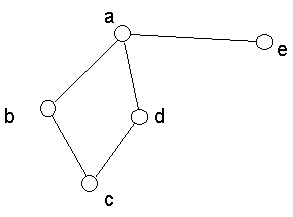
\includegraphics[width=2in]{figures/geodesic-fig.png}

\caption{Distancia Geodésica.}
\label{fig:geodesica}
\end{figure}

En la figura ~\ref{fig:geodesica}  la distancia geodésica entre "e" y "c" es 3 ya que hay que recorrer tres aristas para llegar desde uno nodo al otro.

\subsection{Distancia entre Grafos}

Esta distancia sirve para comparar un grafo con otro, es decir que queremos saber que tan diferentes son dos grafos cualesquiera. La definición es similar a la distancia de edición entre strings, contamos el costo de las operaciones necesarias para convertir un grafo en otro. Las operaciones posibles son agregar un nuevo nodo, eliminar un nodo, agregar una arista o eliminar una arista, todas ellas de costo 1. 

\begin{figure}[!htb]
\centering
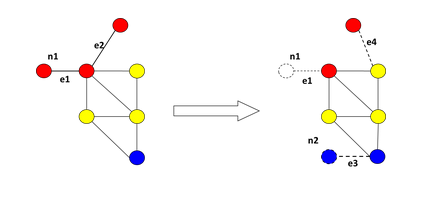
\includegraphics[width=3in]{figures/graph-distance-fig.png}

\caption{Distancia entre grafos.}
\label{fig:graphdistance}
\end{figure}

En la figura ~\ref{fig:graphdistance} vemos dos grafos a distancia 6, ya que para pasar del primero al segundo son necesarias las siguientes operaciones:

\begin{enumerate}
\item eliminar la arista e1
\item eliminar el nodo n1
\item eliminar la arista e2
\item agregar la arista e4
\item insertar el nodo n2
\item insertar la arista e3
\end{enumerate}

\subsection{Distancia para atributos categóricos: VDM}
Hasta el momento no hemos visto ninguna distancia que tenga sentido para atributos categóricos o factores es decir aquellos que pueden tomar un valor de una lista predeterminada de valores. Temas como cuál es la distancia entre "masculino" y "femenino" o entre "rojo" y "verde" no son conceptos para nada claros. Para este tipo de atributos vamos a definir la distancia VDM (value distance measure) de la siguiente forma:

$$VDM(f1,f2) = \sum_{class=i}^{c} |P(f1|class_i)-P(f2|class_i)|$$

Consideremos el siguiente ejemplo en el cual tenemos dos clases: "azul" y "rojo" y un atributo categórico con tres valores posibles: "A","B" o "C". Supongamos los siguientes puntos:

\begin{verbatim}
(rojo,A)
(azul,B)
(rojo,C)
(azul,B)
(azul,C)
\end{verbatim}

Podemos calcular la probabilidad de cada uno de los valores posibles para el atributo en función de cada clase, por ejemplo $P(A|rojo)$ es la probabilidad del atributo "A" si la clase es rojo. Para la clase rojo nuestro atributo toma una vez el valor "A" y una vez el valor "C" por lo tanto $P(A|rojo)=1/2$. La tabla de probabilidades es:

\begin{table}[!hbt]
\center{
\begin{tabular}{|c|c|c|}\hline
 & rojo & azul\\ \hline\hline
A & 1/2 & 0 \\
B  & 0 & 2/3  \\
C & 1/2 & 1/3 \\ \hline
\end{tabular}
}
\vskip 0.25cm
\caption{Probabilidades de factores.}
\end{table}

A partir de esta tabla podemos calcular las distancias A-B, A-C y B-C usando la fórmula de la VDM. Por ejemplo para la distancia entre A y B tenemos que hacer la sumatoria de la diferencia entre la probabilidad de "A" y "B" en cada una de las clases es decir: $VDM(A,B) = |(1/2-0)| + |(0-2/3)| = 1/2 + 2/3 = 7/6$. La tabla de distancias es la siguiente:

\begin{table}[!hbt]
\center{
\begin{tabular}{|c|c|c|c|}\hline
&A &B & l\\ \hline\hline
A & 0 & 7/6 & 1/3 \\
B  & 7/6 & 0 & 5/6  \\
C & 1/3 & 5/6 & 0 \\ \hline
\end{tabular}
}
\vskip 0.25cm
\caption{Ejemplo distancia VDM.}
\end{table}

Es decir que "A" está mas cerca de "C" que de "B" 

\subsection{Distancias Especiales}

En muchos casos es necesario definir una distancia mixta o customizada de acuerdo a la aplicación que tenga nuestro set de datos. Consideremos por ejemplo un set de datos sobre películas, para cada película conocemos su director, género, actores principales, actores de reparto, estudio, año de publicación, guionista, sonidista, etc etc. Es decir que tenemos una buena cantidad de atributos de tipos realmente muy diferentes. La dificultad pasa por calcular la distancia entre dos películas o lo que es lo mismo la semejanza entre dos películas. 

Este tipo de problemas necesitan de la definición de una distancia "custom" o definida por el usuario. Por ejemplo podemos asignar "pesos" a cada uno de los diferentes atributos y posibles valores de semejanza. Si las películas tienen el mismo director entonces 5 puntos, sino 0 puntos. Si no tienen actores en común 0 puntos, 1 punto si tienen un actor en común y 2 puntos si tienen 2 o mas actores en común. Si el año es el mismo 3 puntos, si la diferencia es de 1 o 2 años 2 entre 3 y 5 años 1 punto y mas de 5 años 0 puntos, etc. De esta forma definimos la semejanza máxima que puede haber entre dos películas como el máximo de puntos que podemos sumar cuando todos los atributos son idénticos. Luego la semejanza entre dos películas se puede calcular como la suma de puntos sobre el total posible y la distancia es 1-semejanza ya que la semejanza es un número entre 0 y 1. Esta construcción de distancias o semejanzas "custom" es clave en sistemas de recomendación basados en contenidos en donde queremos recomendarle a un usuario productos similares a aquellos que le han gustado o ha comprado recientemente. Este tema será tratado con mayor extensión en el capítulo sobre sistemas de recomendación.

\subsection{Aprendiendo la Distancia}

Una posibilidad intrigante para la distancia entre los puntos es aprenderla a partir de los puntos mismos. Dados los puntos y la clase a la que pertenece cada uno podemos usar un algoritmo de clasificación conocido como "Random Forests" que será desarrollado mas adelante para aprender un modelo a partir de nuestros datos. En un Random Forest obtenemos un conjunto de $n$ árboles de decisión en donde cada árbol intenta clasificar a nuestros puntos. Tomando dos puntos podemos calcular su distancia como el número de árboles en los que RF predice una clase diferente para cada punto. Normalizando sobre la cantidad de árboles $n$ tenemos una distancia entre 0 y 1. 

Este tipo de distancias que aprendemos con un algoritmo para aplicar luego otro algoritmo deben ser tomadas con cuidado, por ejemplo no tendría sentido aprender una distancia con RF para luego aplicar KNN para clasificar si el resultado del Random Forest es superior al que obtenemos con KNN. 

\section{Determinando la Distancia a usar en KNN}

Tenemos que comentar ahora de que forma determinar la distancia a usar en KNN, el método básico es probando diferentes distancias y viendo cual de ellas nos da un mejor resultado. Dada una cierta distancia de un cierto valor de $k$ podemos ver para cada punto de nuestros datos de entrenamiento, para los cuales conocemos su clase (o valor si es un problema de regresión) cual sería la predicción del algoritmo KNN. Luego simplemente comparamos las predicciones con los valores conocidos para calcular la precisión del algoritmo o el error del mismo. En un problema de clasificación podemos calcular el porcentaje de puntos que el algoritmo clasifica correctamente mientras que en un problema de regresión podemos calcular la sumatoria total de los errores al cuadrado sobre el total de puntos (MSE o Mean Squared Error).

Notemos que la precisión de KNN puede calcularse directamente a partir del set de entrenamiento, en el set de entrenamiento cada punto tiene una clase, lo que hacemos es tomar cada punto y clasificarlo en base a sus $k$ vecinos mas cercanos y comparar esta predicción con la clase real del punto que conocemos. Este mecanismo nos permite analizar el comportamiento de KNN en el set de entrenamiento y nos ayuda a elegir los mejores hiper-parámetros para el algoritmo. Al usar este método de validación cuando tomamos cada punto no lo consideramos como parte de sus k-vecinos, es decir que hacemos de cuenta que el punto está fuera del set de entrenamiento. Si los puntos fueran muchos podemos seleccionar algunos al azar para calcular la precisión del algoritmo (Montecarlo style)

\section{Determinar el valor de K}

Para determinar el valor óptimo para K el procedimiento es igual que para determinar la métrica a usar como distancia: probar diferentes valores de $k$ y ver cual es el que nos da mejores resultados. Aquí hay que tener un cierto cuidado ya hay que entender qué implica aumentar o disminuir la cantidad de vecinos mas cercanos y es la primera vez que encontramos el concepto de sobre-ajuste (overfitting) al cual nos referiremos de aquí en mas como overfitting por ser el término mas comúnmente usado en la literatura para describir el problema.

Veamos qué pasa cuando usamos $k=1$ es decir cuando a cada punto lo clasificamos únicamente en base al punto mas cercano.

\begin{figure}[!htb]
\centering
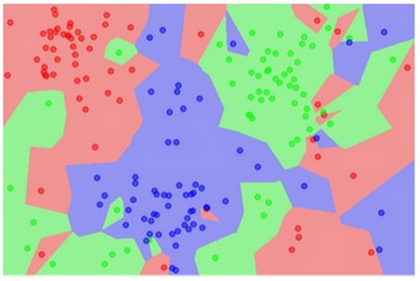
\includegraphics[width=3in]{figures/kn1-fig.png}
\caption{KNN con $k=1$.}
\label{fig14}

\end{figure}

Lo que podemos ver es que la distribución que aprende nuestro clasificador no es homogénea, es decir que hay puntos de distintas clases mezclados en zonas en las cuales predomina otra clase, esto implica que nuestro clasificador va a funcionar bien o muy bien para el set de entrenamiento pero no ha aprendido a generalizar y esto quiere decir que no va a ser muy bueno para predecir la clase de puntos nuevos que no hayamos observado en el set de entrenamiento. Esta es la definición de \textit{overfitting}: cuando un algoritmo funciona bien o muy bien para el set de entrenamiento y mal para datos nuevos. El concepto es que aprender a predecir el set de entrenamiento no es lo mismo que aprender a generalizar. En KNN para generalizar mejor hay que usar valores de $k$ mayores. Veamos qué pasa con $k=5$

\begin{figure}[!htb]
\centering
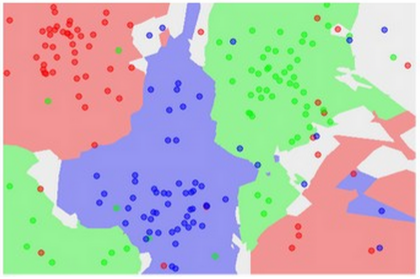
\includegraphics[width=3in]{figures/kn5-fig.png}

\caption{KNN con$ k=5$.}
\label{fig:knn5}
\end{figure}

Como podemos ver en la figura ~\ref{fig:knn5}  el clasificador ha aprendido ahora a generar áreas mas suaves y por consiguiente es un clasificador que generalizará mejor para predecir puntos que no estaban en el set de entrenamiento. Podríamos pensar que es entonces conveniente usar valores de $k$ grandes como $k=1000$ o incluso $k=n$ sin embargo las cosas no son tan sencillas. Al aumentar el valor de $k$ estamos dando cada vez mayor peso a las clases que tienen mayor cantidad de puntos en el set de entrenamiento, en el extremo si $k=n$ vamos a predecir para todos los puntos la clase que mayor cantidad de puntos tiene en el set de entrenamiento lo cual no es bueno. En definitiva el $k$ óptimo en KNN es aquel que nos de un buen desempeño en cuanto a la precisión de clasificación para el mayor $k$ posible. Una forma de encontrar este valor óptimo es seleccionar el mayor $k$ que nos de una precisión aceptable para el problema que estemos trabajando.

Veamos un ejemplo de la precisión de un clasificador de tipo KNN para diferentes valores de $k$

\begin{figure}[!htb]
\centering
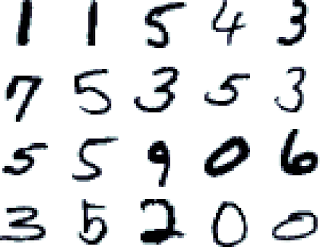
\includegraphics[width=2in]{figures/mnist-fig-1.png}
\caption{MNIST dataset}
\label{fig16}

\end{figure}

En este caso usamos KNN para predecir el valor de dígitos manuscritos en el set de datos MNIST. El set de entrenamiento cuenta con 20.000 imágenes de 28x28 pixeles cada una representando dígitos manuscritos. Cada imagen tiene como clase el dígito que representa (0 a 9). El set de test tiene otras 10.000 imágenes cuya clase no conocemos. Aplicamos KNN para determinar a qué clase corresponde cada dígito en base a la clase de sus $k$ vecinos mas cercanos usando la distancia euclidiana.

\begin{figure}[!htb]
\centering
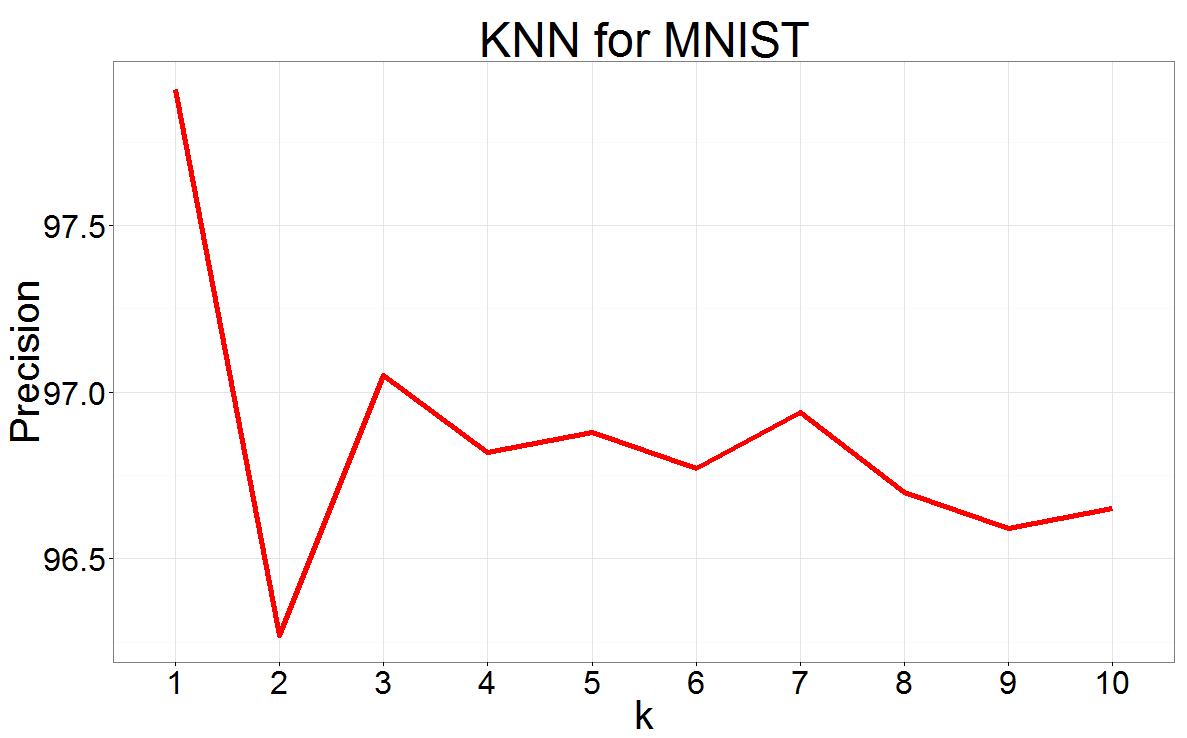
\includegraphics[width=3in]{figures/knn-mnist-fig.png}
\caption{KNN para MNIST}
\label{fig17}

\end{figure}

Observamos en primer lugar que KNN tiene un resultado muy bueno para este set de datos, esto se debe a que el set de datos está presentado de forma ideal para KNN mas adelante explicaremos el motivo. En cuanto al valor de $k$ si  $k=1$ tenemos un caso de overfitting, $k=2$ no funciona nada bien y luego podríamos llegar a elegir prácticamente cualquier valor entre $k=3$ y $k=11$ ya que todos esos valores tienen un muy buen nivel de precisión y también generalizan bien.

\subsection{Grid Search y Random Search en KNN}

En un algoritmo vamos a llamar parámetros a aquellos valores que el algoritmo encuentra a partir de los datos y vamos a llamar hiper-parámetros a aquellos datos que el algoritmo necesita para poder funcionar. KNN tiene dos hiper-parámetros: $k$ y la métrica a usar (distancia). Para encontrar los hiper-parámetros óptimos para un algoritmo pueden usarse dos métodos: Grid-Search o Random-Search. En un Grid-Search probamos todas las combinaciones posibles dentro de una lista de valores posibles para cada hiper parámetro. Si por ejemplo probamos cuatro métricas y diez valores de k, tenemos que correr KNN un total de 40 veces. Es posible empezar con un "paso" grueso para los hiper parámetros y luego ir refinando la búsqueda, por ejemplo podemos probar primero con $k=1,5,10,15,20$ y luego si el óptimo resultó ser por ejemplo 10 buscar entre $k=6 $ $k=14$. Este proceso es especialmente necesario cuando los hiper-parámetros pueden tomar valores reales.

\begin{algorithm}
 \KwData{X: training set, Y: labels,m:number of observations}
 \KwResult{k and distance metric for KNN }
$best\_precision = 0$, $best\_k=0$,$ best\_metric=none$\;
 \For{k in (1..100)}{
 \For {metric in (euclidean,manhattan, cosine, jaccard,hamming,linf,...)} {
  preds = knn(X,Y,k,metric)\;
  precision = sum(preds==Y)/m\;
\If{$precision >best\_precision$}{
   best\_precision = precision\;
   best\_k = k\;
   best\_metric = metric \;
   }
}
}
 \caption{Grid Search for KNN}
\end{algorithm}

Cuando la cantidad de hiper-parámetros es realmente muy grande la combinatoria a realizar puede resultar muy ineficiente, en estos casos puede recurrirse al método de Random-Search. En un Random-Search controlamos cuantas iteraciones realizamos de nuestro algoritmo y por cada iteración seleccionamos los valores de los hiper-parámetros al azar dentro de un rango pre-establecido. Este método no es tan preciso como un grid-search pero es mucho mas rápido.Random-Search es nuestro primer ejemplo de algoritmo aleatorizado una rama de los algoritmos que usaremos extensamente en el curso.

\section{Sensibilidad a valores fuera de escala}

Es hora de hablar de los puntos débiles de KNN y qué tipo de cosas pueden hacer que el algoritmo tenga malos resultados. Un primer factor importante es que dado que KNN se basa en distancias para funcionar correctamente, queremos que todos los atributos de nuestros datos tengan el mismo peso en el cálculo de distancias, si los atributos no están todos dentro de la misma escala entonces puede que un atributo domine el cálculo de distancias sobre todos los demás y el algoritmo tendrá un rendimiento pobre. 

Para evitar que un atributo domine el cálculo de distancias es necesario normalizar los valores de los atributos (columnas), por ejemplo al rango [0..1]. Esto se logra restándole a cada atributo el promedio de la columna y luego dividiendo por la desviación standard de la misma. Al restar el promedio logramos que el promedio de la columna sea cero y al dividir por la desviación standard logramos que el rango sea [0..1]. A este procedimiento lo llamaremos "Normalización de atributos o features" o simplemente "Normalización". Son muchos los algoritmos que necesitan datos normalizados para funcionar mejor. Notemos que normalizar no cambia las propiedades geométricas de los datos es decir que las distancias se mantienen.

\section{Sensibilidad a atributos anómalos}

Mas allá de haber normalizado los datos es posible que no todos los atributos sean adecuados para clasificar. Consideremos por ejemplo un caso muy simple en el cual estamos intentando predecir la altura de alumnos en base a otros datos como el peso, edad, sexo, etc. Atributos del estilo "educación" o el promedio en la carrera o las notas que tenga claramente no son relevantes para la tarea que estamos desarrollando. En muchos casos esto no es evidente ya que desconocemos cuáles son los atributos mas relevantes y cuáles son no-relevantes de acuerdo a lo que queremos predecir. Los algoritmos de Forward Selection y Backward Selection permiten determinar cuál es el conjunto de atributos óptimo para KNN.

\subsection{Forward Selection}

En el algoritmo de forward selection comenzamos con cero atributos y en cada paso agregamos el atributo que mejor resultado nos genera. Para considerar el resultado podemos usar un valor fijo para $k$ o bien la mejor precisión para varios valores de $k$ o bien un promedio de la precisión para diferentes valores de $k$ probados.
De esta forma vamos iterando y agregando atributos siempre y cuando los resultados mejoren, cuando ya no es posible mejorar los resultados o bien cuando no quedan mas atributos por agregar termina el algoritmo y tenemos el set de atributos a usar en KNN. 

\begin{algorithm}[]
 \KwData{data:X, labels:Y, number of observations:m}
 \KwResult{Set of features to use}
unused\_features=[all features], used\_features=[], best\_precision = 0\;
 \While{not empty unused\_features}{
  loop\_precision = 0\;
  best\_at = NULL\;
  \For{at in unused\_features} {
  pred = knn(X[used\_features + at],Y,k,metric)\;
  precision = sum(pred==Y)/m\;
  \If{$precision > loop\_precision$} {
    loop\_precision = precision\;
    best\_at = at;
  }
  }
  \eIf{$loop\_precision > best\_precision$}{
   add best\_at to used\_features\;
   remove best\_at from unused\_features\;
   best\_precision = loop\_precision\;
   }{
   EXIT \#No improvement adding any feature\\
  }
 }
 \caption{Forward Selection}
\end{algorithm}

\subsection{Backward Selection}

Backward selection es la versión inversa del algoritmo forward selection. Comenzamos con todos los features y vamos eliminando un feature a la vez hasta que ya no se pueda mejorar la precisión del algoritmo. 

\begin{algorithm}[]
 \KwData{data:X, labels:Y, number of observations:m}
 \KwResult{Set of features to use}
  used\_features=[all\_features], best\_precision = 0\;
 \While{True}{
  loop\_precision = 0\;
  best\_at = NULL\;
  \For{at in used\_features} {
  pred = knn(X[used\_features - at],Y,k,metric)\;
  precision = sum(pred==Y)/m\;
  \If{$precision > loop\_precision$} {
    loop\_precision = precision\;
    best\_at = at;
  }
  }
  \eIf{$loop\_precision > best\_precision$}{
   remove best\_at from used\_features\;
   best\_precision = loop\_precision\;
   }{
   EXIT \#No improvement removing any feature\\
  }
 }
 \caption{Backward Selection}
\end{algorithm}

\section{Aproximaciones para KNN}

\subsection{Orden del algoritmo y eficiencia}

Es necesario ahora analizar la eficiencia del algoritmo KNN, en su versión mas simple para clasificar un punto nuevo tenemos que compararlo contra todos los puntos existentes ($m$) para encontrar los $k$ vecinos mas cercanos. Cada una de estas $m$ comparaciones implica comparar $n$ dimensiones. Por lo tanto el orden del algoritmo es $O(m*n)$

La necesidad de comparar cada punto a clasificar contra todos los puntos del set de datos es el gran problema de KNN y el motivo por el cual suele ser muy ineficiente para datos masivos. Clasificar 1000 puntos con un set de entrenamiento de un millón de datos implicaría un total de mil millones de comparaciones cada una de ellas en $n$ dimensiones. Esto nos lleva a la conclusión de que KNN no escala bien y que a partir de una cierta cantidad de datos es necesario usar algún tipo de optimización o aproximación que nos permita lograr mejores resultados. Veremos a continuación algunas de estas posibles optimizaciones y aproximaciones.

\subsection{Indices Espaciales: KD-Trees}

Un índice espacial es una estructura de datos en donde podemos insertar nuestros puntos n-dimensionales de forma tal de luego poder realizar búsquedas de los puntos mas cercanos a un cierto query sin tener que recorrer todos los puntos del set de datos. Existen muchísimas variantes de estos índices, a efectos de ejemplo vamos a mencionar el mas popular que son los llamados KD-Trees. Por motivos que vamos a aclarar muy pronto vamos a ser muy breves en cuanto a la descripción del funcionamiento de un KD-Tree.

Un KD-Tree es similar a un árbol binario de búsqueda pero en cada nivel del árbol comparamos una coordenada diferente de nuestros puntos n-dimensionales. Si trabajamos en dos dimensiones la raíz del árbol compara la coordenada "X" del punto, todos los puntos con X menor al valor de la raíz van a la rama izquierda y todos los puntos con X mayor o igual al valor de la raíz van a la rama derecha. En el siguiente nivel comparamos la coordenada Y. Todos los puntos con Y menor al valor del nodo van a la izquierda y los mayores o iguales a la derecha. En el siguiente nivel volvemos a la coordenada "X" y así sucesivamente hasta que cada rama tenga un solo punto o bien hasta un máximo número de niveles prefijados.

Conociendo los puntos a insertar podemos tomar como valor de "split" en cada nivel al punto para el cual la coordenada con la cual estamos trabajando es la media. La mediana funciona mejor que el promedio porque nos permite siempre dividir el conjunto de puntos en dos partes mas o menos iguales y eso logra que el árbol quede balanceado lo cual es fundamental para que la búsqueda dentro del mismo sea de orden logarítmico y no lineal.

\begin{figure}[!htb]
\centering
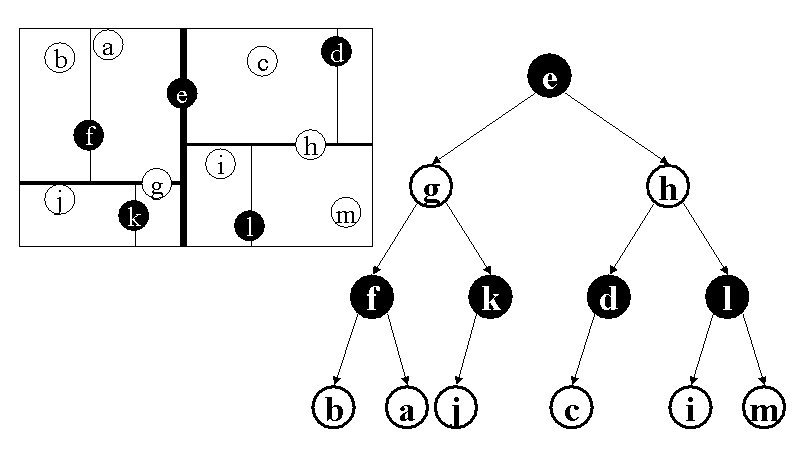
\includegraphics[width=5in]{figures/kdtree-fig.png}

\caption{KD-Tree en 2D}
\label{fig:kdtree2d}
\end{figure}

La figura ~\ref{fig:kdtree2d} nos muestra un KD-Tree en dos dimensiones y la forma en la cual el árbol particiona el espacio. La representación que se obtiene se llama "treemap" y es una visualización popular para datos que se presentan de forma jerárquica como los árboles, carpetas en un disco, etc.

Un KD-Tree permite buscar los puntos mas cercanos a un query sin tener que recorrer todos los puntos del set de datos, comenzando por la raíz vamos navegando el árbol de acuerdo a las coordenadas del punto que buscamos, eventualmente hace falta hacer algo de backtracking para obtener los $k$ vecinos mas cercanos al punto pero en general se trata de una operación de orden logarítmico, eso es bueno y en principio podríamos pensar que un KD-Tree o algún otro de los índices espaciales es la solución ideal al problema de la búsqueda de los vecinos mas cercanos para el algoritmo KNN. Sin embargo esto no es así.

El problema de los KD-Trees y de todos los índices espaciales en general es que sólo funcionan bien para muy pocas dimensiones, 2, 3 o 4 dimensiones. A medida que la cantidad de dimensiones aumenta los índices degradan muy rápidamente a punto tal de ser iguales a la simple comparación por fuerza bruta contra todos los puntos. Este problema es una versión del meta-problema conocido como "la maldición de la dimensionalidad" del cual hablaremos mas adelante pero que ya podemos definir de una forma muy simple: "algunos algoritmos no funcionan bien con muchas o muy pocas dimensiones". En este caso los índices espaciales sólo funcionan bien con muy pocas dimensiones. Es por esto que no les dedicamos mucho espacio ni dedicación ya que es muy raro contar con un problema de Data Science en el cual los datos se presenten en dos o tres dimensiones. Los índices espaciales son muy útiles en aplicaciones gráficas, juegos y todo tipo de programas en los cuales trabajemos en dos o tres dimensiones, lamentablemente no es nuestro caso. Mas adelante al hablar de dimensionalidad vamos explicar mejor el motivo por el cual los KD-Trees degradan a una búsqueda lineal cuando tenemos muchas dimensiones.

\subsection{Indices Espaciales: VP-Trees}

Los VP-Trees son otra forma de índice espacial, también sufren la maldición de la dimensionalidad pero resisten mucho mas a la misma que un KD-tree, es decir que si un índice espacial nos va a ayudar a que KNN funcione mas rápido lo mas probable es que dicho índice sea un VP-Tree.

Un VP-Tree debe su nombre a (Vantage Point Tree) y afortunadamente es una estructura de datos muy sencilla que no necesita de ningún parámetro, el único detalle crucial es que la métrica usada para las distancias en KNN debe cumplir sí o sí con la desigualdad triangular.

Vamos a comentar primero como se construye un VP-Tree y luego como usarlos para resolver el problema de los vecinos mas cercanos a un cierto punto.

Empezamos considerando a todos los puntos en un único nodo. Elegimos al azar un punto que será nuestro "Vantage Point" inicial. Calculamos la distancia desde dicho punto a todos los demás y calculamos la mediana de todas las distancias. Luego dividimos los puntos en dos conjuntos: aquellos cuya distancia es menor o igual a la mediana y aquellos cuya distancia es mayor a la media. La raíz del árbol contiene el Vantage-Point (punto elegido), la mediana de las distancias que llamaremos $\mu$ y dos punteros uno al sub-árbol izquierdo con todos los puntos a distancia menor o igual a la mediana y otro al sub-árbol derecho con todos los puntos con distancia mayor a la media. Este proceso se repite recursivamente hasta que queda formado el árbol. 

\begin{figure}[!htb]
\centering
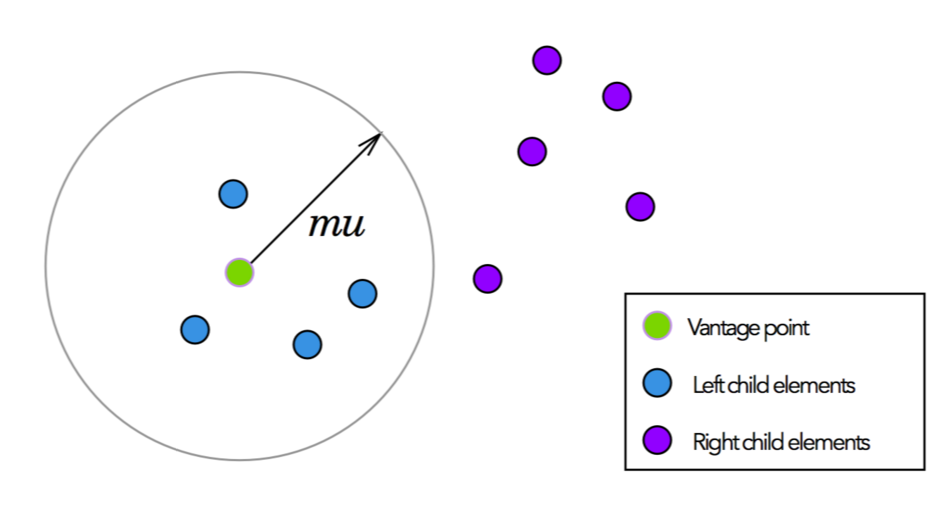
\includegraphics[width=3in]{figures/vptree.png}

\caption{VP-Tree}
\label{fig:vptree}
\end{figure}

Cuando queremos realizar un query empezamos por la raíz. Si la distancia desde el punto query $q$ a la raíz ($\tau$) es menor a $\mu$ entonces calculamos si con un radio de $\tau$ estamos siempre dentro del radio de $\mu$ alrededor del punto raíz. Si esto ocurre solo tenemos que explorar la rama izquierda del árbol usando la distancia entre el query y la raíz como valor para $\tau$. 

Si con un radio de $\mu$ alrededor del punto query quedamos siempre fuera del círculo de radio $\mu$ alrededor de la raíz entonces solo tenemos que explorar el sub-árbol derecho usando $\tau=\mu$

En el peor caso estamos en un caso intermedio entre los dos anteriores y tenemos que explorar ambos sub-árboles. 

Una vez que accedemos al sub-árbol izquierdo o derecho analizamos la distancia entre el punto query y esta raíz y repetimos el proceso.

\begin{figure}[!htb]
\centering
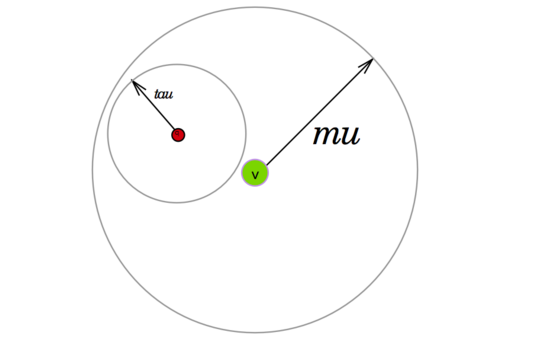
\includegraphics[width=2in]{figures/vptree1.png}

\caption{VP-Tree caso en el cual solo recorremos el sub-árbol izquierdo}
\label{fig:vptree1}
\end{figure}

\begin{figure}[!htb]
\centering
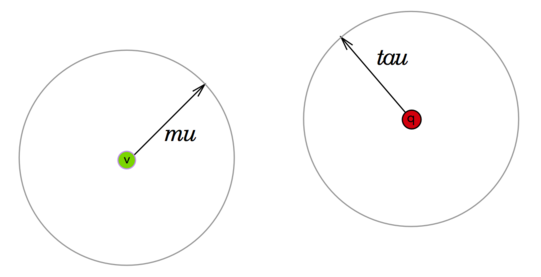
\includegraphics[width=2in]{figures/vptree2.png}

\caption{VP-Tree caso en el cual visitamos solo el sub-árbol derecho}
\label{fig:vptree2}
\end{figure}

\begin{figure}[!htb]
\centering
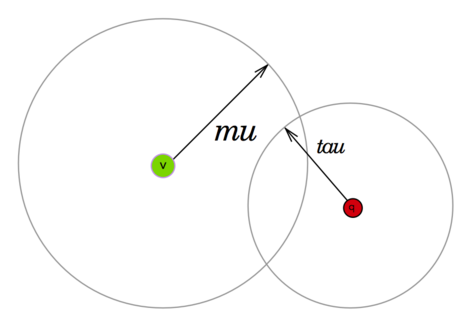
\includegraphics[width=2in]{figures/vptree3.png}

\caption{VP-Tree caso en el cual visitamos ambos sub-árboles}
\label{fig:vptree3}
\end{figure}

Los VP-Trees son sencillos de construir y usar y suelen ser los índices espaciales que mejor resisten la maldición de la dimensionalidad. Notemos que el proceso de construcción del árbol es extremadamente simple y que para usar el árbol para resolver queries solo hace falta lógica para determinar en que hijos visitar de cada nodo y cuando podemos detener la búsqueda al ya tener $k$ puntos cercanos al query y estar seguros de que no puede haber mas. El árbol tiene toda la información necesaria para poder hacer esto.

Si bien los VP-Trees son superiores (en general) a los KD-Trees no son perfectos y cuando trabajos con muchas dimensiones puede darse que en todos los casos haya que recorrer los dos hijos de cada nodo lo cual degrada en una búsqueda lineal o peor (por el overhead). Esto ocurre rapidamente en datos sintéticos y aleatorios, incluso con pocas dimensiones pero como los datos reales nunca son random podemos suponer que no se distribuyen de forma uniforme por lo que un VP-Tree puede darnos una ventaja cuando la cantidad de puntos con la que estamos trabajando es realmente muy grande incluso en muchas dimensiones. Esto nos muestra que existe una puja constante entre la maldición de la dimensionalidad y la bendición de la no-uniformidad de los datos y diferentes algoritmos explotan esta tensión de forma diferente.

\subsection{Líderes y seguidores}

El algoritmo de líderes y seguidores es un algoritmo aleatorizado para aproximar el problema de los $k$ vecinos mas cercanos. Este algoritmo necesita de una etapa de pre-procesamiento de los datos que se hace una única vez y luego de esta permite aproximar los vecinos mas cercanos sin necesidad de comparar contra todos los puntos. El algoritmo es bastante sencillo y lo describimos a continuación.

En primer lugar tomamos una cantidad de puntos al azar de nuestro set de datos, en general $\sqrt{n}$ y los denominamos "líderes". Luego procesamos cada uno de los puntos que quedaron del set de datos y comparando contra cada líder lo asignamos al líder mas cercano. De esta forma luego de la etapa de pre-procesamiento cada punto del set de entrenamiento o bien es un líder o bien está asociado (linkeado) a un líder. 

Para buscar los $k$ vecinos mas cercanos a un cierto query lo que hacemos es buscar comparar el punto contra cada líder y para el líder mas cercano comparar contra todos sus seguidores. Es decir que hacemos únicamente comparaciones con $2*\sqrt{n}$ puntos ya que suponemos que cada líder tiene asociados en promedio $\sqrt{n}$ seguidores.  Es evidente que este algoritmo es una aproximación ya que puede ocurrir que los $k$ puntos encontrados no sean exactamente los $k$ vecinos mas cercanos, tal vez un punto mas cercano estaba asociado a otro líder y se nos escapa de la búsqueda. Es posible "tunear" la precisión de este algoritmo sacrificando velocidad por mayor precisión, una forma de hacer esto es comparar contra los $n$ líderes mas cercanos en lugar de uno solo.

\begin{algorithm}[]
 \KwData{data:X, labels:Y, number of observations:m}
 \KwResult{set of leaders}
  leaders = randperm(m)[1..$\sqrt{m}$]\;
 \For{point in X}{
  \If{point not in leaders}{
   compare point against each leader\;
   assign point to closest leader\;
   }
 }
 \caption{Lideres y seguidores: pre-procesamiento}
\end{algorithm}

\begin{algorithm}[]
 \KwData{query: Q data:X, leaders:L,k,metric}
 \KwResult{$k$ closest neighbors}
 l = findClosestLeader(Q,L)\;
candidates = findPointsByLeader(X,l)\;
neigbors = KNN(Q, candidates, k, metric)\;
 \caption{Lideres y seguidores:query}
\end{algorithm}

\subsection{Aproximación con K-Means}

\begin{figure}[!htb]
\centering
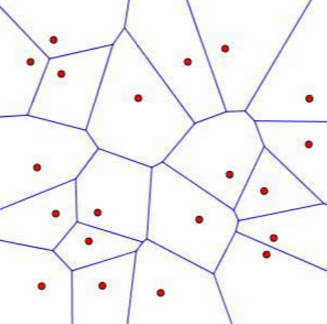
\includegraphics[width=2in]{figures/vorono-fig-1.png}

\caption{Diagrama de Voronoi en 2D representando los centroides de K-Means}
\label{fig:vorono}
\end{figure}

Una opción muy similar al método de líderes y seguidores es aplicar K-Means a los datos tomando $\sqrt{m}$ centroides ($m$ es la cantidad de puntos). K-Means es un algoritmo de clustering que veremos mas adelante que nos devuelve un conjunto de centroides y a cada punto lo asigna al centroide mas cercano, igual que en líderes y seguidores. 

Cuando queremos los $k$ vecinos mas cercanos a un punto comparamos contra los centroides y los puntos que pertenecen a ese cluster. Eventualmente podemos comparar contra los $b$ centroides mas cercanos si queremos mejor precisión con el costo de algunas comparaciones mas.

Este método difiere de líderes y seguidores en que los líderes no son ahora puntos tomados al azar sino los centroides encontrados por K-Means por lo que es mas probable que se distribuyan mejor en el espacio de nuestros datos. La desventaja es que tenemos que correr K-Means sobre el set de datos lo cual es menos eficiente que simplemente tomar los líderes al azar. 

Dependiendo del caso uno u otro método pueden funcionar muy bien para aproximar el problema. 

\subsection{Editing}

El proceso conocido como "editing" en KNN consiste en eliminar del set de entrenamiento puntos que no son necesarios para la clasificación de otros puntos. Consideremos que para un cierto valor fijo de $k$ nuestro espacio de puntos definido por el set de entrenamiento queda dividido en áreas que corresponden a cada una de las clases posibles, cualquier punto futuro que caiga dentro de cada área será clasificado con la clase que corresponde al área dentro de la cual ha caído el punto.

\begin{figure}[!htb]
\centering
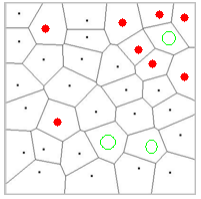
\includegraphics[width=2in]{figures/knn-voronoi-fig.png}
\caption{KNN fronteras}
\label{fig19}

\end{figure}

Notemos que para definir cada área sólo es necesario contar con los puntos que están cerca de las fronteras de las mismas, los puntos interiores no juegan ningún papel en la clasificación de puntos  cuya clase desconocemos. El proceso de editing tiene como objetivo eliminar dichos puntos. Los puntos que son realmente relevantes para clasificar los vamos a llamar \textit{prototipos} nuestro objetivo es encontrar los prototipos y descartar el resto de los puntos.

Para encontrar los prototipos hay dos procedimientos, uno parecido a forward selection y el otro a backward selection solo que en lugar de features estaremos seleccionando instancias (puntos).

En forward-edit comenzamos con un conjunto vacío de puntos, luego por cada punto de nuestro set de datos nos fijamos si el punto quedaría correctamente clasificado con los puntos que tenemos hasta el momento, si el punto queda correctamente clasificado entonces lo descartamos mientras que si queda mal clasificado entonces es necesario cambiar la frontera por lo que agregamos el punto al conjunto de prototipos.

\begin{algorithm}[]
\KwData{data:X,k,metric}
\KwResult{T:set of prototypes}
$T={}$ \\
\For{point  x in X} {
 \If{x is NOT correctly classfied in T} {
    add point x to T\\
 }
}
\caption{Forward Editing}
\end{algorithm}

La versión llamada backward-editing comienza con todos los puntos. Luego por cada punto del conjunto verificamos si al removerlo el punto igual quedaría bien clasificado en cuyo caso removemos al punto del conjunto. El resultado final es el set de prototipos.

\begin{algorithm}[]
\KwData{data:X,k,metric}
\KwResult{T:set of prototypes}
$T=X$ \\
\For{point x in T} {
 \If{x is correctly classfied in T-\{x\}} {
    remove point x from T\\
 }
}
\caption{Backward Editing}
\end{algorithm}

El proceso de editing mejora la performance de KNN y no cambia en absoluto la precisión del algoritmo para clasificar ya que solo remueve de nuestro set de entrenamiento aquellos puntos que no son necesarios para clasificar. El costo es la necesidad de pre-procesar todos los puntos para obtener los prototipos tarea que sólo debemos realizar una única vez. 

\subsection{NN vía Grafos}

Es posible usar grafos para construir una estructura de datos que nos permita aproximar el problema de los $k$ vecinos mas cercanos de forma eficiente. Para construir el grafo es necesario realizar un pre-procesamiento de los datos. Cada punto será un nodo del grafo y lo vamos a linkear a sus $k$ vecinos mas cercanos. Esto implica hacer una pasada de KNN para todos los puntos del set de entrenamiento, podemos combinar esta pasada con el proceso de editing y eliminar puntos redundantes o ruidosos al mismo tiempo. El resultado del pre-procesamiento es entonces un grafo con tantos nodos como puntos y donde cada nodo tiene $k$ aristas.

\begin{figure}[!htb]
\centering
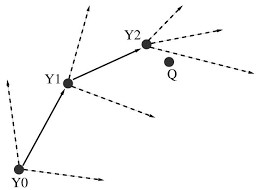
\includegraphics[width=2in]{figures/knn-graphs-fig.png}

\caption{KNN aproximado por grafos}
\label{fig:knngrafos}
\end{figure}

Para buscar los $k$ puntos mas cercanos a un cierto query lo que hacemos es comenzar desde un punto al azar del grafo y calcular la distancia entre el query y los vecinos de dicho punto. Una vez que hicimos esto nos movemos al nodo que mas nos acerca al query. Este proceso lo repetimos hasta que no hay posibilidad de acercarnos mas al query. En el camino nos quedamos con los $k$ puntos que hayan estado mas cerca del query que estamos procesando. 
En la figura ~\ref{fig:knngrafos} si empezamos en Y0 y nuestro Query es Q nos movemos primero a Y1 y luego a Y2 guardando siempre en el camino cuáles son los $k$ puntos mas cercanos a Q de los que hemos analizado. Por cada nodo visitado siempre analizamos sus $k$ vecinos.
Este algoritmo es bastante rápido y eficiente siempre y cuando sea factible realizar el pre-procesamiento necesario.[Dong][Hajebi]

\subsection{LSH}

LSH (Locality Sensitive Hashing) es un conjunto de algoritmos para determinar rápidamente datos que son similares entre sí, la idea es usar una función de hashing especial de forma tal que si dos datos son similares la función de hashing los asigne a una misma posición o bucket. Es fácil entender cómo estas funciones pueden usarse para aproximar el algoritmo KNN en lo que denominaremos ANN (Approximate Nearest Neighbors), por cada punto simplemente aplicamos la función de hashing y comparamos contra todos los puntos que estén dentro del bucket indicado. Esto permite aproximar los $k$ vecinos mas cercanos a un cierto punto en $O(1)$ lo cual es extremadamente eficiente. 
LSH  puede usarse con diferentes métricas y es un tema tan importante que mas adelante le dedicaremos un capítulo completo. Por el momento sepamos que LSH es una de las formas mas eficientes para aproximar el problema de los vecinos mas cercanos a un punto. 

\section{Teoría de KNN}

\begin{framed}
\begin{quote}
"Here be dragons"
\end{quote}
\end{framed}

Esta es la sección mas teórica del capítulo en donde vamos a desarrollar el error que comete KNN al clasificar. Para empezar debemos plantear cuál es el error mínimo que puede tener un clasificador que llamaremos $e^*$, para entender este error supongamos que tenemos un set de datos en el cual todos los puntos tienen exactamente los mismos atributos pero diferente clase. Esta claro que lo mejor que podemos hacer es $1-P(C)$ siendo "C" la clase mayoritaria. Si tenemos dos clases, una con el 70\% de los puntos y otra con el 30\% entonces nuestro error será de 0.3. El error siempre lo vamos a calcular como un número entre 0 y 1 que es la probabilidad de que clasifiquemos mal un punto. Si todos los puntos son iguales lo mejor que podemos hacer es predecir la clase mayoritaria para todos los puntos y nuestro error será igual a la proporción de puntos que no están en esta clase.
Vamos a analizar ahora cuál es el error cometido por KNN cuando $k=1$ es decir que clasificamos únicamente en base al vecino mas cercano, llamemos a este algoritmo NN. (por nearest neighbor). 

\subsection{Teorema de Cover-Hart}

\begin{theorem}[Cover-Hart]
Si $e^*$ es el error óptimo de un clasificador entonces si tenemos infinitos datos el error de NN es $eNN \leq 2 e^*$
\end{theorem}

Supongamos únicamente dos clases (+)  y (-).

$$ eNN = P^+ * PNN^- + P^- * PNN^+$$

Dejando todo en función de los positivos:

$$ eNN = P^+  *  (1-PNN^+) + (1-P^+) * PNN^+$$

Es decir que el error cometido por NN es igual a la probabilidad de que el punto sea positivo por la probabilidad de que NN lo clasifique como negativo mas la probabilidad de que el punto sea negativo por la probabilidad de que NN lo clasifique como positivo.

Veamos qué pasa cuando tenemos infinitos puntos es decir $n\to\infty$

$$\lim_{n\to\infty} PNN^+ = P^+$$
$$\lim_{n\to\infty} PNN^- = P^-$$

Esto vale ya que con infinitos puntos la probabilidad que NN califique a un punto como positivo es exactamente igual a la proporción de puntos positivos en el set de datos que es $P^+$

Por lo tanto con infinitos puntos podemos reescribir el error de NN como:

$$eNN = P^+*(1-P^+) + (1-P^+)*P^+$$

Supongamos ahora que $P^+$ es la clase minoritaria, ya que es lo mismo suponer que es $P^+$ o $P^-$. Si $P^+$ es la clase minoritaria entonces $e^*=P^+$ y podemos entonces escribir el error de NN en función de $e^*$

$$eNN = 2 e^*(1-e^*) \leq 2e^*$$

Esta última fórmula es la desigualdad de Cover-Hart y es muy importante ya que nos asegura que NN tiene en el peor de los casos el doble de error que un clasificador ideal, esto puede parecer mucho si el error ideal es 0.3 porque NN podría llegar a errar en el 60\% de los casos pero cuando el error ideal es bajo como por ejemplo 0.01 NN no puede ser peor que 0.02.

Una conclusión interesante de la desigualdad es que si el error óptimo es $e^*$ y el error de KNN con $k=1$ es a lo sumo $2e^*$ entonces cuando tomamos $k>1$ nuestro mejor resultado es a lo sumo el doble de tomar $k=1$. En otras palabras si con $k=1$ tenemos un error de 0.14 entonces lo mejor que podemos obtener con cualquier otro valor de $k$ es un error de 0.07. Esta es una cota extremadamente importante ya que permite probar métricas con $k=1$ y luego analizar cuanto pueden mejorar tomando mayor cantidad de vecinos.

La desigualdad de Cover-Hart puede extenderse a KNN y lo que obtenemos es que para KNN el error es a lo sumo el error ideal multiplicado por una constante "c" muy chica, esto quiere decir que si los datos fueran infinitos KNN sería óptimo. Hay que tener cuidado al interpretar esto ya que los datos \textbf{nunca} son infinitos y por mas grande que sea el conjunto de datos la diferencia entre infinito y un número muy grande es infinito. Por lo tanto no podemos decir que con muchos datos KNN sea óptimo. 

La conclusión que sí podemos obtener es que KNN mejora a medida que tenemos mayor cantidad de puntos, cuanto mejor definidas queden las fronteras mejor será la performance del algoritmo en clasificar puntos nuevos. 

\section{Parzen Windows}

El algoritmo Parzen Windows es un familiar muy cercano de KNN, en lugar de seleccionar siempre los $k$ vecinos mas cercanos Parzen Windows selecciona los vecinos que están dentro de una cierta distancia $\sigma$ prefijada. Esto lleva a que la cantidad de vecinos a considerar sea variable.

\begin{figure}[!htb]
\centering
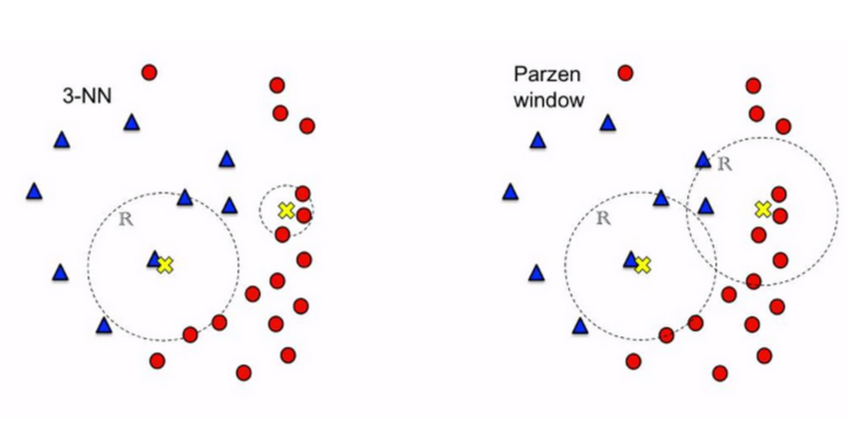
\includegraphics[width=4in]{figures/knn-parzen-fit.png}
\caption{KNN vs Parzen Windows}
\label{fig:parzen}

\end{figure}

La figura ~\ref{fig:parzen} muestra la diferencia existente entre Parzen Windows y KNN, en uno es variable la cantidad de vecinos y fija la distancia y en el otro se fija la cantidad de vecinos y las distancias son variables.
En cuanto a los resultados obtenidos en general ambos algoritmos dan resultados bastante similares, Parzen Windows suele usarse mas para problemas de regresión que para clasificación aunque los motivos teóricos para que esto ocurra nunca han sido expuestos.

\section{KNN con pesos}

Una extensión lógica al algoritmo KNN es darle pesos a los vecinos de acuerdo a su proximidad con respecto al punto que queremos estimar. Esto es especialmente lógico en problemas de regresión en donde podemos razonar que si nuestro punto está realmente muy cerca de otro entonces el valor a estimar debería ser muy parecido al de dicho punto sin que vecinos mas alejados influyan mucho.Notemos que el uso de pesos invalida el proceso de editing ya que ahora todos los puntos del set de entrenamiento pueden ser útiles.

La idea es entonces asignar a cada uno de los $k$ vecinos un peso $W_i$ que vamos a calcular de la siguiente forma:

$$W_{i \ne 1} = \frac{d(x,x_k) - d(x,x_i)}{d(x,x_k)-d(x,x_1)}$$

Con la salvedad de que el punto mas cercano tiene siempre peso igual a 1 y el mas lejano tiene peso 0. $x_k$ es el vecino mas lejano, $x_1$ es el vecino mas cercano.

Por ejemplo supongamos que $k=5$ y las distancias que tenemos son (ordenadas de menor a mayor): (3,3.25,6,7,13).

Para el primer punto el peso es igual a 1 por definición. Para el segundo punto el peso lo calculamos de la forma:

$$W_2 = \frac{13-3.25}{13-3} =0.975$$

Mientras que para el cuarto punto el peso es:

$$W_4 = \frac{13-7}{13-3} = 0.6$$

Una vez que calculamos los pesos es sencillo estimar el valor de regresión para el punto en cuestión como:

$$\bar{Y} = \frac{\sum_i W_i * X_i}{\sum_i Wi}$$

Notemos que también podemos usar este esquema para problemas de clasificación. En KNN antes cada vecino tenía un voto para determinar a que clase pertenece el punto, ahora tendrá el valor correspondiente a $W_i$ y la clase que sume mas es la que determina la clase del nuevo punto.

Otra forma popular de "pesar" los vecinos en KNN es mediante la fórmula:

$$W_i = \frac{1}{d(x,x_i)^\beta}$$

En donde $\beta$ es un parámetro. Cuando $\beta=0$ tenemos el algoritmo tradicional, todos los puntos tienen peso = 1. Cuando $\beta=1$ tenemos una interpolación lineal, cuando $\beta=2$ le damos un peso cada vez menor a los puntos que se alejan del punto original.

Finalmente una tercera opción es pesar los puntos mediante un gaussiano alrededor de cada punto:

$$W_i = \exp(-\frac{|x_i-x|^2}{2\sigma^2})$$

$\sigma$ es el radio alrededor de cada punto para considerar que los puntos dentro del mismo son vecinos. Podemos determinar $\sigma$ calculando el promedio de las distancias entre cada punto y su k-ésimo vecino mas cercano.

Un detalle muy interesante es que al usar pesos podemos usar un valor de $k$ tan grande como deseemos, los puntos mas lejanos simplemente van a tener un peso cada vez menor y en concreto podríamos usar $k=n$ en cuyo caso para clasificar un punto tenemos en cuenta todos los puntos del set de datos como vecinos. Cuando esto pasa lo que tenemos es efectivamente un \textit{kernel} de distancias entre puntos. Mas adelante al ver otros algoritmos de clasificación dedicaremos un buen tiempo al estudio de métodos basados en kernels.

Existen otros esquemas interesantes para usar pesos en KKN descriptos en [Gou]

\section{Evitando Overfitting en KNN}

En KNN, y especialmente cuando $k$ es un número chico, existe el riesgo de overfitting, es decir que el algoritmo funcione muy bien para el set de entrenamiento pero no tan bien para puntos nuevos, esto es un error de generalización.

Una forma de evitar el error de generalización consiste en eliminar del set de entrenamiento puntos anómalos definiendo como punto anómalo aquel para el cual todos sus vecinos pertenecen a una clase diferente a la del punto. Luego de eliminar los puntos anómalos la capacidad de generalizar del algoritmo debería ser superior ya que se elimina el efecto de estos puntos en la frontera de algoritmo. Este proceso es compatible con el proceso de edición, es posible al mismo tiempo que buscamos los prototipos eliminar los puntos anómalos.

\section{RKNN: Ensambles basados en KNN}

Es posible combinar el resultado de varios algoritmos KNN en un ensamble. Hemos mencionado que KNN es muy sensible a cuáles son los atributos (features) que usamos para calcular las distancias, podemos entonces crear un ensamble en donde cada KNN usará un conjunto de $m$ atributos al azar de nuestro set de datos.

Por ejemplo si tenemos 5 atributos: (A,B,C,D,E) si usamos $m=3$ podemos tener un KNN que use (A,C,D) otro con (B,C,E) otro con (A,B,D), etc. Cada KNN va a realizar una predicción para el set de test o bien para cada punto de nuestro set de datos (leave one out cross validation), la predicción del ensamble surge de cuál es la opinión mayoritaria de todos los KNN. En un problema de clasificación binaria si tenemos un total de 100 KNNs y 82 de ellos dicen que un punto es de clase "1" y los otros 18 dicen que es de clase "0" entonces vamos a clasificar al punto como de clase "1" con probabilidad 0.82. 

La cantidad de atributos $m$ es un hiper-parámetro al igual que $k$ y la métrica a usar como distancia, los tres hiper-parámetros tienen que buscarse por grid-search usando cross-validation. 

El uso de un ensamble permite minimizar el impacto de atributos que no son buenos predictores o que afectan el resultado de KNN, un detalle muy importante es que el ensamble nos permite calcular la importancia predictora de cada atributo. Cada KNN tiene un cierto promedio de precisión, que podemos extenderle a cada uno de los atributos que participan del mismo, por lo tanto podemos promediar el promedio de precisión de cada atributo simplemente calculando la precisión de los KNN en los cuáles el atributo participa. Por ejemplo:

\begin{table}[!hbt]
\center{
\begin{tabular}{|l|l|}\hline
\textbf{Atributos} & \textbf{Precisión} \\ \hline
A,C,D & 0.78\\
A,B,E & 0.84\\
B,C,D & 0.81\\
C,D,E & 0.75\\ \hline
\end{tabular} 
}
\caption{Ejemplo de un ensamble de 4 KNNs con 3 atributos sobre un total de 5}
\end{table}

En este caso el atributo "A" tiene una precisión promedio de 0.81, "B" tiene 0.825, "C" tiene 0.78 y "D" tiene 0.78. Esto lo podemos usar para detectar cuáles son los atributos que ayudan mas a KNN y cuáles son los menos significativos y eliminarlos, realizando un nuevo ensamble con menor cantidad de atributos posibles. Este es un caso de feature-selection basado en un ensamble de KNNs.

\section{Algunas conclusiones y comentarios}

KNN es un algoritmo extremadamente importante. Es capaz de funcionar tanto para problemas de clasificación como para problemas de regresión y se ajusta perfectamente a fronteras no-lineales. Requiere el ajuste de únicamente dos hiper-parámetros que son el valor de $k$ (si no usamos pesos) y la métrica a usar para determinar las distancias. A mayor cantidad de puntos en el set de entrenamiento mejor es el resultado de KNN y en el límite si los puntos fueran infinitos KNN es óptimo en el sentido de minimizar el error de clasificación. Irónicamente KNN, en su versión mas \textit{naive} escala muy mal al tener que calcular las distancias contra todos los puntos del set de datos por cada punto a clasificar. Vimos varios algoritmos y métodos para hacer que KNN sea mas eficiente ya sea reduciendo la cantidad de puntos contra los cuales tenemos que calcular las distancias o usando algoritmos de aproximación que sólo usan un subconjunto del set de entrenamiento para clasificar. Los índices espaciales que funcionan muy bien en pocas dimensiones degradan en la búsqueda por fuerza bruta en espacios de dimensiones medianos a grandes por lo que en general no los usamos para KNN, nos referimos a esto como un caso de la maldición de la dimensionalidad y este es el tema de nuestra próxima sección.

\section{Dimensionalidad}

Estudiar la dimensionalidad de los datos es un paso fundamental, imprescindible en la mayoría de los procesos de Data Science. Este estudio implica entender en que espacio se presentan los datos, en que espacio residen realmente, cómo se comportan los algoritmos que pretendemos usar en estos espacios y si resulta conveniente realizar alguna transformación del espacio original a otro espacio a efectos de lograr algún beneficio. 

\subsection{Manifolds}
Un Manifold es un espacio que localmente se comporta como un espacio euclideano aunque globalmente no lo sea. El mejor ejemplo que podemos dar para ilustrar esto es el de una esfera como nuestro planeta mismo. En una esfera la distancia euclideana no funciona, sin embargo una pequeña porción de la esfera puede tratarse como un espacio euclideano y es así como medimos las distancias con las cuales nos manejamos diariamente. Para ir desde un punto de una ciudad a otro nadie tiene en cuenta que se está moviendo sobre la superficie de una esfera.

\begin{figure}[!htb]
\centering
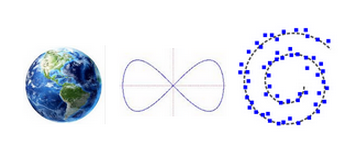
\includegraphics[width=3in]{figures/manifolds-fig.png}

\caption{Manifolds}
\label{fig:manifoldocho}
\end{figure}

Un ejemplo de algo que no es un Manifold es la figura de ocho que mostramos en el centro de la figura ~\ref{fig:manifoldocho}. En este espacio los puntos en el "cruce" nunca se comportan como un espacio euclideano sin importar que tan chica sea la escala en la cual se trabaje. 

En muchos casos un conjunto de datos se presenta en un espacio que no corresponde a la dimensionalidad real de los datos, cuando tenemos un espacio representado en otro hablaremos de un "embedding", este puede ser de mayor o menor cantidad de dimensiones que el espacio original. La espiral a la derecha de la figura ~\ref{fig:manifoldocho} es un buen ejemplo de esto, lo que tenemos es un Manifold unidimensional en un espacio de dos dimensiones. Si tomamos una pequeña porción de la espiral los puntos se comportan localmente bajo las reglas de un espacio euclideano y podríamos estirar la espiral hasta quedarnos con una recta que representaría a nuestros datos perfectamente. A los algoritmos que intentan descubrir la verdadera dimensionalidad de los datos los llamaremos algoritmos de "Manifold Learning", una categoría muy importante dentro de Data Science. 

\subsection{Los Datos No son Random y Siempre Tienen Pocas Dimensiones}

Este concepto es fundamental y muchas veces se lo ignora lo cual lleva a realizar todo tipo de afirmaciones incorrectas e incluso a predecir de forma totalmente infundada el comportamiento de un algoritmo. La premisa que intentaremos explicar es que independientemente de la cantidad de dimensiones en las cuales se presenten los datos estos casi siempre tienen pocas dimensiones. Es decir que frecuentemente nuestros datos se van a presentar como un manifold de pocas dimensiones inmerso en un espacio dimensional mucho mayor. Algo semejante a lo que sería una superficie de dos dimensiones en un espacio tridimensional.

\begin{figure}[!htb]
\centering
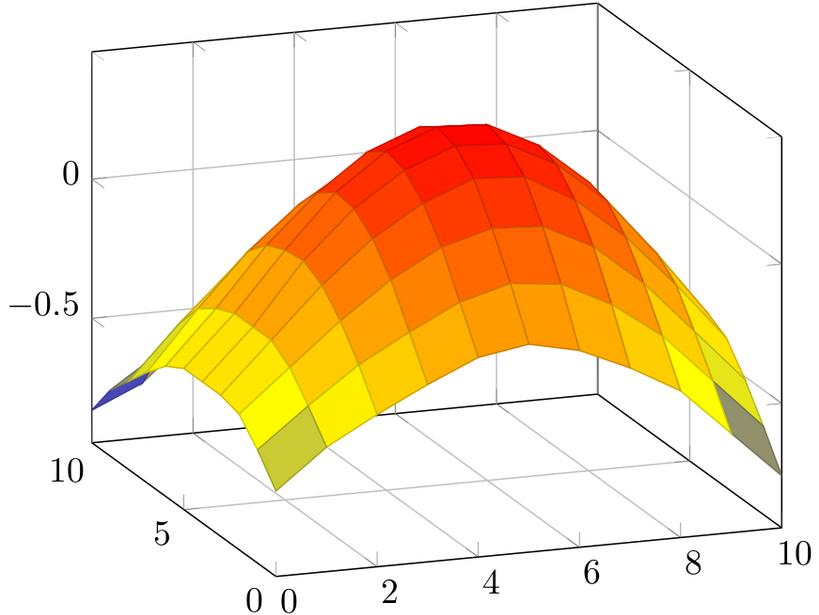
\includegraphics[width=3in]{figures/2dmanifold-fig.png}
\caption{Manifold de 2d en 3d}

\end{figure}

Para explicar por qué decimos que los datos siempre tienen pocas dimensiones la clave es entender que los datos no son aleatorios, si fueran aleatorios no serían datos sino ruido. Que los datos tengan un significado, que sean entendibles por un ser humano implica que existe una estructura en los mismos y esto implica que no sean aleatorios. Como los datos no son aleatorios es imposible que "cubran" todo el espacio dimensional en el cual se presentan. Empecemos con un ejemplo muy simple: Datos sobre personas para las cuales registramos la altura y peso. Estos datos se presentan en 2d pero no ocupan el espacio total en 2d, por ejemplo una persona que mide 1 metro 50 no puede pesar 1345kg y una persona que pesa 55kg no puede medir 4 centímetros. 

Otro ejemplo muy claro son las imágenes, supongamos que tenemos un set de datos con imágenes de 32x32 pixeles en blanco y negro. Está claro que nuestros datos se presentan en un espacio de 1024 dimensiones (32x32) pero también debe quedar claro que nuestras imágenes de ninguna forma cubren la totalidad de dicho espacio, esto es porque no cualquier vector de 1024 pixeles es una imagen válida.

\begin{figure}[!htb]
\centering
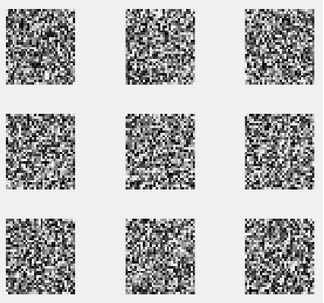
\includegraphics[width=3in]{figures/random-images-fig.png}
\caption{Imágenes aleatorias}

\end{figure}

Las imágenes al azar que mostramos no tienen ningún sentido y nunca formarían parte de nuestro set de datos, por ejemplo si las imágenes fueran fotos podríamos argumentar que no son fotos posibles. Esto quiere decir que sólo un subespacio de nuestro espacio de 1024 dimensiones contiene las imágenes que serían válidas, aquellas que tienen sentido. En otras palabras las imágenes se presentan en un manifold de una cierta cantidad de dimensiones inmerso en un espacio de 1024 dimensiones. 

\subsection{Manifold Learning y Cambios de Dimensiones}

Los algoritmos de manifold learning y cambio de dimensiones permiten transformar los datos de un espacio dimensional a otro, para hacer esto tiene que existir algún motivo válido, es decir una razón que explique por qué nos conviene trabajar en un espacio de dimensiones que no es aquel en el cual se presentaron los datos originalmente. Algunos motivos muy comunes son:

\begin{enumerate}
\item Para poder visualizar los datos en dos o tres dimensiones. (¡este es un motivo poderoso!)
\item Porque el algoritmo que queremos usar funciona mejor en otro espacio dimensional. (combatir la maldición de la dimensionalidad)
\item Por razones de eficiencia de tiempo o espacio
\item Para eliminar el ruido de nuestro set de datos
\end{enumerate}

En mayor o menor medida es probable que uno o varios de estos motivos se presenten en nuestras aplicaciones. Es por esto que casi siempre vamos a tener que usar de una forma u otra algún algoritmo de cambio de dimensiones. Existen muchos algoritmos para cambiar las dimensiones de los datos y vamos a dedicarles un capítulo entero mas adelante.

\subsection{La Maldición de la dimensionalidad}

Este tema es muy popular y lamentablemente en una enorme cantidad de sitios, blogs, apuntes e incluso libros está incorrectamente definido y explicado, vamos a intentar explicar de qué se trata realmente la "maldición" y por qué se presta a confusión. 

La definición que vamos a usar para la maldición de la dimensionalidad es muy simple: "no todos los algoritmos se comportan bien en cualquier espacio de dimensiones". Algunos algoritmos se comportan bien en pocas dimensiones y otros se comportan mejor en muchas dimensiones. Hemos estudiado KNN y hemos visto que si trabajamos en pocas dimensiones podemos usar un índice espacial, podríamos decir entonces que la maldición de la dimensionalidad para KNN pasa por no poder usar índices espaciales y tener que caer en una búsqueda por fuerza bruta u otros recursos cuando las dimensiones son muchas. Es importante entender que para cada algoritmo hay razones completamente diferentes por las cuales podemos preferir muchas o pocas dimensiones. 

Habiendo hecho esta definición tan genérica y mostrado un ejemplo conocido que ya hemos estudiado podríamos dar por cerrado el tema, sin embargo, es conveniente mostrar algunos efectos de tener muchas o pocas dimensiones y cómo a veces estos efectos pueden llevar a alguna confusión acerca de su influencia en el funcionamiento de los algoritmos.

\subsubsection{El problema del muestreo}

En todo problema de Data Science es correcto decir que cuantos mas datos podamos recolectar mejor serán nuestros resultados. Esto es algo lógico ya que los datos ayudan a que nuestros algoritmos puedan entenderlos y generar mejores resultados. En 2001 Banko y Brill [Banko,Brill] publicaron un trabajo que se hizo muy famoso en el cual sostenían que en la mayoría de los casos recolectar mas datos era mas importante que usar un algoritmo mejor. Dicho de otra forma con cantidad de datos suficientes incluso algoritmos muy simples convergen al mismo resultado que los algoritmos mas avanzados.

\begin{figure}[!htb]
\centering
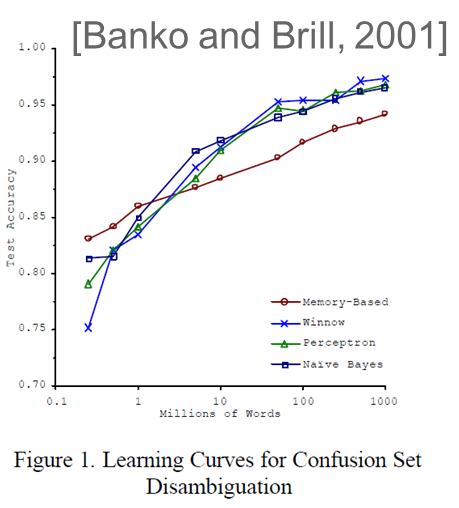
\includegraphics[width=3in]{figures/banko-brill-fig.png}
\caption{Banko and Brill 2001}

\end{figure}

Una vez que hemos establecido que a mayor cantidad de datos mejores resultados tenemos que analizar el efecto de la dimensionalidad en la cantidad de datos necesarios. Es fácil darse cuenta que a medida que aumenta la cantidad de dimensiones del set de datos aumenta exponencialmente la cantidad de datos "posibles" por lo tanto a mayor cantidad de dimensiones necesitamos exponencialmente mas datos para mantener el mismo nivel de muestreo (sampling). 

Podemos decir entonces que este es uno de los efectos de la maldición de la dimensionalidad sin embargo tenemos que ser muy cuidadosos, es cierto que a mayor cantidad de dimensiones la cantidad de datos "posibles" aumenta exponencialmente si y sólo si cualquier dato es "posible" pero esto implicaría datos aleatorios y hemos establecido que los datos nunca son aleatorios. Por lo tanto hay que tener mucho cuidado al decir que a mayor cantidad de dimensiones necesitamos muchos mas datos para tener un buen muestreo, en la mayoría de los casos con datos reales esta afirmación no es válida.

\subsection{El Efecto de la Dimensionalidad sobre las Distancias}
Es necesario estudiar el efecto que la dimensionalidad tiene sobre las distancias, en concreto sobre la distancia general de Minkowsky que definimos como:

$$d(x,y)=(\sum |x-y|^p)^{1/p}$$

Como vivimos en un mundo tridimensional algunos efectos que ocurren al tomar distancias en espacios de muchas dimensiones pueden parecer completamente contra-intuitivos, algunos ejemplos de estos curiosos efectos son:

\begin{itemize}
\item En un espacio de muchas dimensiones si tenemos una distribución gaussiana multinomial la mayoría de la masa no está en la mediana de la distribución sino en una cáscara alrededor de la misma.
\item En muchas dimensiones la mayor parte del volumen de una hiper-esfera está en su superficie y no dentro de la misma (!)
\item En muchas dimensiones los puntos dentro de un hipercubo están mas cerca de la frontera del hipercubo que de su vecino mas cercano
\item En muchas dimensiones la distancia euclideana entre puntos tiende a converger
\end{itemize}

Estos curiosos efectos nos llevan a la conclusión de que debemos tener mucho cuidado al trabajar en espacios multidimensionales y a pensar que la selección de una métrica adecuada puede ser fundamental, por ejemplo para el funcionamiento de un algoritmo como KNN que está basado en distancias.

El efecto de la dimensionalidad en las distancias queda evidenciado por el siguiente teorema:

\begin{theorem}[Beyer]
$$if \lim_{d  \to \infty} var(\frac{||x||_d}{E[||x||_d]}) = 0, then \frac{Dmax-Dmin}{Dmin} \to 0$$
\end{theorem}

La demostración de este teorema puede encontrarse en [Beyer] y lo que nos dice es que a medida que la cantidad de dimensiones tiende a infinito la diferencia entre la distancia máxima entre dos puntos del espacio y la distancia mínima converge es decir que todas las distancias son aproximadamente iguales. Este es un resultado muy perturbador. Afortunadamente, como hemos visto, los datos reales no suelen ocupar completamente el espacio en el cual se presentan pero de todas formas es importante considerar que en muchas dimensiones el concepto de distancia entre puntos empieza a peligrar.

Consideremos el caso de la norma $l_{\infty}$ es decir la diferencia máxima que existe entre x e y en alguna dimensión. Esta norma es útil en dos o tres dimensiones pero es claro que a medida que aumentamos la cantidad de dimensiones su utilidad va decreciendo, en un espacio de 100 dimensiones por ejemplo la diferencia máxima en solo una de estas dimensiones ciertamente no debe ser la mejor forma de medir la distancia entre dos puntos. La intuición es que a medida que aumentamos la cantidad de dimensiones exponentes cada vez mas bajos nos dan una mejor medida de distancia entre los puntos, este razonamiento es cierto y fue demostrado tanto en forma teórica como empírica en [Aggarwal,Hinnenburg,Keim]. Se demuestra que para espacios de muchas dimensiones la distancia Manhattan ($p=1$) funciona mejor que la distancia euclideana e incluso distancias con $p<1$ funcionan aun mejor. 

\begin{figure}[!htb]
\centering
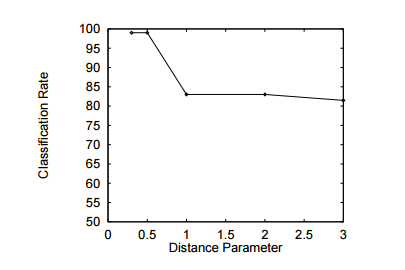
\includegraphics[width=3in]{figures/distancias-fig.png}
\caption{Comportamiento de distancias en un algoritmo de clasificación para 20 dimensiones}

\end{figure}

La conclusión es que en espacios multidimensionales debemos considerar distancias con exponentes bajos, incluso menores a 1 y darles la oportunidad de competir contra la distancia euclideana comparando los resultados porque en muchos casos nos vamos a encontrar con que las distancias con exponentes fraccionarios y menores a uno tienen un rendimiento superior en algoritmos de clasificación y clustering.

\subsubsection{El problema de los KD-Trees}

Retomamos ahora el problema de los KD-Trees en muchas dimensiones, hemos dicho que en muchas dimensiones un KD-Tree degrada en una búsqueda por fuerza bruta, vamos a intentar una explicación intuitiva de por qué sucede esto. 

Nuestro espacio de $d$ dimensiones se puede ver como un hipercubo, consideremos una hiper-esfera inscripta dentro del hipercubo. A medida que la cantidad de dimensiones aumenta el volumen de la esfera se vuelve insignificante con respecto al volumen del hipercubo. Esto es muy fácil de ver pensando en que porcentaje de superficie ocupa un círculo inscripto dentro de un cuadrado y que porcentaje de volumen ocupa una esfera inscripta dentro de un cubo.

\begin{figure}[!htb]
\centering
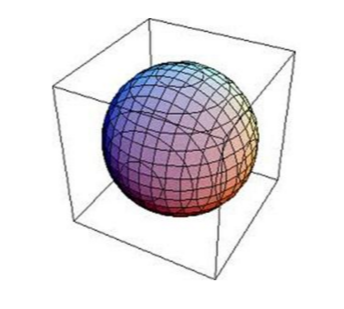
\includegraphics[width=2in]{figures/dimcurse-fig-1.png}
\caption{Distancias y dimensionalidad}

\end{figure}

Esta observación sirve para sacar algunas conclusiones interesantes: cuando trabajamos en muchas dimensiones la mayoría de los puntos se concentra en las esquinas del hipercubo y por lo tanto la distancia entre los puntos se vuelve muy parecida. Este es el motivo por el cual un KD-tree se degrada, como las distancias son todas muy parecidas no es posible elegir un split en cada dimensión de forma tal que estemos seguros que el punto mas cercano a nuestro query está de un lado del split y no del otro. En forma intuitiva es como si en cada split del KD-Tree no pudiéramos tomar una decisión ya que para un punto dado el punto mas cercano podría estar en cualquier dirección, por lo tanto no queda otra que considerar prácticamente todos los puntos y por eso los KD-Trees y cualquier índice espacial degrada cuando tenemos muchas dimensiones. 

\subsubsection{Shared Neighbors}

Además del uso de exponentes fraccionarios hay otros trucos que podemos probar cuando trabajamos en muchas dimensiones, uno de estos trucos es el concepto de "vecinos mas cercanos compartidos" o (Shared nearest neighbors). Esta métrica define la distancia entre dos puntos x e y como la intersección entre los vecinos mas cercanos de ambos puntos.

$$SNN(x,y) = |KNN(x,k) \cap KNN(y,k)|$$

Esta métrica ha demostrado funcionar mejor que otras en espacios de muchas dimensiones. [Houle]

